% !TEX root = ../main.tex

\section{Normal forms}
\label{sec:normalforms}

In this section we provide normal forms for the logics $\ofo$, $\ofoe$ and 
$\ofoei$. 
These normal forms will be pivotal for characterising the different fragments of 
these logics in later sections.
\begin{convention}
Here and in the sequel it will often be convenient to blur the distinction 
between lists and sets.
For instance, identifying the list $\vlist{T} = T_{1}\cdots T_{n}$ with the
set $\{ T_{1}, \ldots, T_{n} \}$, we may write statements like $S \in \vlist{T}$ 
or $\Pi \subseteq \vlist{T}$. 
Moreover, given a finite set $\Phi = \{\phi_1, \dots, \phi_n\}$, we write $\phi_1 \land \dots \land \phi_n$ as $\bigwedge \Phi$, and $\phi_1 \lor \dots \lor \phi_n$ as $\bigvee \Phi$. If $\Phi$ is empty, we set as usual $\bigwedge \Phi = \top$ and $\bigvee \Phi = \bot$.
Finally, notice that we write $\bigvee_{1\leq m < m^{\prime} \leq n} (y_m \foeq y_{m^{\prime}}) \lor \psi$ as $\arediff{\vlist{y}} \to \psi$. 
\end{convention}

%%%
%%% NF for OFO
%%%

\subsection{Normal form for $\ofo$}

We start by introducing a normal form for monadic first-order logic without 
equality.

\begin{definition}\label{def:bfofo}
Given sets of types $\Sigma, \Pi \subseteq \wp(A)$, we define the following 
formulas:
\[\begin{array}{lll}
   \dgbnfofo{\Sigma}{\Pi} &\isdef&
   \bigwedge_{S\in\Sigma} \exists x. \tau_S(x) \land 
   \forall x. \bigvee_{S\in\Pi} \tau_S(x)
\\ \dbnfofo{\Sigma}      &\isdef& \dgbnfofo{\Sigma}{\Sigma}
\end{array}\]
A sentence of $\ofo(A)$ is in \emph{basic form} if it is 
a disjunction of formulas of the form $\dbnfofo{\Sigma}$.
\end{definition}

Clearly the meaning of the formula $\dbnfofo{\Sigma}$ is that $\Sigma$ is a 
complete description of the collection of types that are realised in a monadic 
model. 
Notice that $  \dgbnfofo{\Sigma}{\Pi} = \dbnfofo{\Sigma} = \forall x. \bot$, for 
$\Sigma =\Pi = \nada$.

\medskip

\noindent
Every $\ofo$-formula is effectively equivalent to a formula in basic form.

\begin{fact}\label{fact:ofonormalform}
There is an effective procedure that transforms an arbitrary $\ofo$-sentence 
$\phi$ into an equivalent formula $\tbas{\phi}$ in basic form.
\end{fact}

This observation is easy to prove using Ehrenfeucht-Fra\"iss\'e games -- proof
sketches can be found in~\cite[Lemma 16.23]{ALG02} 
and~\cite[Proposition 4.14]{Venema2014} --, and the decidability of the satisfiability problem for $\ofo$ (Fact \ref{f:decido}). 
We omit a full proof because it is very similar to the following more complex 
cases.


%%%
%%% NF for OFOE
%%%

\subsection{Normal form for $\ofoe$}

When considering a normal form for $\ofoe$, the fact that we can `count types'
using equality yields a more involved basic form.



\begin{definition}
We say that a formula $\phi \in \ofoe(A)$ is in \emph{basic form} if
$\phi = \bigvee \dbnfofoe{\vlist{T}}{\Pi}$ where each disjunct is of the
form
\begin{equation*}
\dbnfofoe{\vlist{T}}{\Pi} = 
\exists \vlist{x}.\big(\arediff{\vlist{x}} \land \bigwedge_i \tau_{T_i}(x_i) 
  \land \forall z.(\arediff{\vlist{x},z} 
  \to \bigvee_{S\in \Pi} \tau_S(z))\big)
\end{equation*}
%
such that $\vlist{T} \in \wp(A)^k$ for some $k$ and $\Pi \subseteq \vlist{T}$.
\end{definition}

We prove that every sentence of monadic first-order logic with equality is
equivalent to a formula in basic form. 
Although this result seems to be folklore, we provide a detailed proof because 
some of its ingredients will be used later, when we give a normal form for 
$\ofoei$. 
We start by defining the following relation between monadic models.

\begin{definition}
For every $k \in \bbN$ we define the relation $\sim^=_k$ on the class $\umods$
of monadic models by putting
\begin{eqnarray*}
\osmodel \sim^=_k \osmodel' \Longleftrightarrow 
  \forall S\subseteq A \ \big(
    |S|_\osmodel = |S|_{\osmodel'} < k \text{ or } 
    |S|_\osmodel,|S|_{\osmodel'} \geq k 
    \big),
\end{eqnarray*}
where $\osmodel$ and $\osmodel'$ are arbitrary monadic models. 
\end{definition}

Intuitively, two models are related by $\sim^=_k$ when their type information 
coincides `modulo~$k$'.
Later on we prove that this is the same as saying that they cannot be 
distinguished by a sentence of $\ofoe$ with quantifier rank at most $k$. 
As a special case, observe that any two monadic models are related by 
$\sim^{=}_{0}$.

For the moment, we record the following properties of these relations.

\begin{proposition}\label{props:eqrelofoe} The following hold:
\begin{enumerate}
\itemsep 0 pt
\item\label{props:eqrelofoe:i} 
The relation $\sim^=_k$ is an equivalence relation of finite index.
\item\label{props:eqrelofoe:ii} 
Every $E \in \umods/{\sim^=_k}$ is characterised by a sentence $\phi^=_E \in 
\ofoe(A)$ with $\qr(\phi^=_E) = k$.
\end{enumerate}
\end{proposition}

\begin{proof}
We only prove the second statement,
and first we consider the case where $k=0$.
The equivalence relation $\sim^{=}_{0}$ has the class $\umods$ of all monadic 
models as its unique equivalence class, so here we may define $\phi^{=}_{\umods}
\isdef \top$.

From now on we assume that $k>0$.
Let $E \in \umods/{\sim^=_k}$ and let $\osmodel \in E$ be a representative. 
Call $S_1,\dots,S_n \subseteq A$ to the types such that $|S_i|_\osmodel = n_i< k$
and $S'_1,\dots,S'_m \subseteq A$ to those satisfying $|S'_i|_\osmodel \geq k$. 
Note that the union of all the $S_i$ and $S'_i$ yields all the possible 
$A$-types, and that if a type $S_{j}$ is not realised at all, we take $n_j = 0$. 
Now define
\begin{align*}
\phi^=_E \quad \isdef \quad  
   & \bigwedge_{i\leq n} \Big(\exists x_1,\dots,x_{n_i}.
   \arediff{x_1,\dots,x_{n_i}} \ \land \ \bigwedge_{j\leq n_i} \tau_{S_i}(x_j)
\\ & \qquad\qquad\qquad \land 
   \forall z. \arediff{x_1,\dots,x_{n_i},z} \to \lnot\tau_{S_i}(z)\Big)\ 
\\ & \land \bigwedge_{i\leq m} \big(\exists x_1,\dots,x_k.\arediff{x_1,\dots,x_k} \land
    \bigwedge_{j\leq k} \tau_{S'_i}(x_j) \big),
\end{align*}
%
where we understand that any conjunct of the form $\exists x_1,
\dots,x_{l}.\psi$ with $l = 0$ is simply omitted (or, to the same effect, 
defined as $\top$).
It is easy to see that $\qr(\phi^=_E) = k$ and that $\osmodel' \models 
\phi^=_E$ iff $\osmodel' \in E$. 
Intuitively, $\phi^=_E$ gives a specification of $E$ ``type by type''; 
in particular observe that $\phi^=_\emodel \equiv \forall x. \bot$.
\end{proof}

Next we recall a (standard) notion of Ehrenfeucht-Fra\"{\i}ss\'e game for 
$\ofoe$ which will be used to establish the connection between ${\sim^=_k}$ and 
$\equiv_k^{\ofoe}$.

\begin{definition}
Let $\osmodel_0 = (D_0,V_0)$ and $\osmodel_1 = (D_1,V_1)$ be monadic models. 
We define the game $\efgame^=_k(\osmodel_0,\osmodel_1)$ between \abelard and 
\eloise.
If $\osmodel_i$ is one of the models we use $\osmodel_{-i}$ to denote the other
model. 
A position in this game is a pair of sequences $\vlist{s_0} \in D_0^n$ and 
$\vlist{s_1} \in D_1^n$ with $n \leq k$. 
The game consists of $k$ rounds where in round $n+1$ the following steps are 
made:
\begin{enumerate}[1.]
\itemsep 0 pt \parsep 0 pt
\item \abelard chooses an element $d_i$ in one of the $\osmodel_i$;
\item \eloise responds with an element $d_{-i}$ in the model $\osmodel_{-i}$.
\end{enumerate}
%
In this way, the sequences $\vlist{s_i} \in D_i^n$ of elements chosen up to 
round $n$ are extended to ${\vlist{s_i}' \isdef  \vlist{s_i}\cdot d_i}$. 
Player \eloise survives the round iff she does not get stuck and the function
$f_{n+1}: \vlist{s_0}' \mapsto \vlist{s_1}'$ is a partial isomorphism of monadic 
models. 
Finally, player \eloise wins the match iff she survives all $k$ rounds.

Given $n\leq k$ and $\vlist{s_i} \in D_i^n$ such that $f_n:\vlist{s_0}\mapsto
\vlist{s_1}$ is a partial isomorphism, we write $\efgame_{k}^=(\osmodel_0,
\osmodel_1)@(\vlist{s_0},\vlist{s_1})$ to denote the (initialised) game where 
$n$ moves have been played and $k-n$ moves are left to be played.
\end{definition}

\begin{proposition}\label{prop:connofoe}
The following are equivalent:
\begin{enumerate}
\itemsep 0 pt \parsep 0 pt
\item\label{prop:connofoe:i} $\osmodel_0 \equiv_k^{\ofoe} \osmodel_1$,
\item\label{prop:connofoe:ii} $\osmodel_0 \sim_k^= \osmodel_1$,
\item\label{prop:connofoe:iii} \eloise has a winning strategy in 
   $\efgame_k^=(\osmodel_0,\osmodel_1)$.
	\end{enumerate}
\end{proposition}
\begin{proof}
Step~(\ref{prop:connofoe:i}) to~(\ref{prop:connofoe:ii}) is direct by
Proposition~\ref{props:eqrelofoe}. 
For~(\ref{prop:connofoe:ii}) to~(\ref{prop:connofoe:iii}) we give a winning 
strategy for \eloise in $\efgame_k^=(\osmodel_0,\osmodel_1)$ by showing the 
following claim.
	%
\begin{claimfirst}
Let $\osmodel_0 \sim_k^= \osmodel_1$ and $\vlist{s_i} \in D_i^n$ be such that
$n<k$ and $f_n:\vlist{s_0}\mapsto\vlist{s_1}$ is a partial isomorphism; then 
\eloise can survive one more round in 
$\efgame_{k}^=(\osmodel_0,\osmodel_1)@(\vlist{s_0},\vlist{s_1})$.
\end{claimfirst}

\begin{pfclaim}
Let \abelard pick $d_i\in D_i$ such that the type of $d_i$ is $T \subseteq A$. 
If $d_i$ had already been played then \eloise picks the same element as before
and $f_{n+1} = f_n$.
If $d_i$ is new and $|T|_{\osmodel_i} \geq k$ then, as at most $n<k$ elements 
have been played, there is always some new $d_{-i} \in D_{-i}$ that \eloise can 
choose to match $d_i$. 
If $|T|_{\osmodel_i} = m < k$ then we know that $|T|_{\osmodel_{-i}} = m$. 
Therefore, as $d_i$ is new and $f_n$ is injective, there must be a $d_{-i} \in 
D_{-i}$ that \eloise can choose. 
\end{pfclaim}
	
Step~(\ref{prop:connofoe:iii}) to~(\ref{prop:connofoe:i}) is a standard
result~\cite[Corollary 2.2.9]{fmt} which we prove anyway because we will need 
to extend it later. 
We prove the following loaded statement.
\begin{claim}
Let $\vlist{s_i} \in D_i^n$ and $\phi(z_1,\dots,z_n) \in \ofoe(A)$ be such 
that $\qr(\phi) \leq k-n$. 
If \eloise has a winning strategy in the game 
$\efgame_k^=(\osmodel_0,\osmodel_1)@(\vlist{s_0},\vlist{s_1})$ then 
$\osmodel_0 \models \phi(\vlist{s_0})$ iff 
$\osmodel_1 \models \phi(\vlist{s_1})$.
\end{claim}
	
\begin{pfclaim}
If $\phi$ is atomic the claim holds because of $f_n:\vlist{s_0}\mapsto 
\vlist{s_1}$ being a partial isomorphism. 
The Boolean cases are straightforward.
Let $\phi(z_1,\dots,z_n) = \exists x. \psi(z_1,\dots,z_n,x)$ and suppose
$\osmodel_0 \models \phi(\vlist{s_0})$. 
Hence, there exists $d_0 \in D_0$ such that $\osmodel_0 \models 
\psi(\vlist{s_0},d_0)$.
By hypothesis we know that \eloise has a winning strategy for 
$\efgame_k^=(\osmodel_0,\osmodel_1)@(\vlist{s_0},\vlist{s_1})$. 
Therefore, if \abelard picks $d_0\in D_0$ she can respond with some $d_1\in D_1$ 
and have a winning strategy for 
$\efgame_{k}^=(\osmodel_0,\osmodel_1)%
@(\vlist{s_0}{\cdot}d_0,\vlist{s_1}{\cdot}d_1)$.
By induction hypothesis, because $\qr(\psi) \leq k- (n+1)$, we have that 
$\osmodel_0 \models \psi(\vlist{s_0},d_0)$ iff $\osmodel_1 \models 
\psi(\vlist{s_1},d_1)$ and hence 
$\osmodel_1 \models \exists x.\psi(\vlist{s_1},x)$. 
The opposite direction is proved by a symmetric argument. 
\end{pfclaim}

\noindent
We finish the proof of the proposition by combining these two claims.
\end{proof}

\begin{theorem}
\label{thm:bnfofoe}
There is an effective procedure that transforms an arbitrary $\ofoe$-sentence 
$\phi$ into an equivalent formula $\tbas{\phi}$ in basic form.
\end{theorem}

\begin{proof}
Let $\qr(\psi) = k$ and let $\ext{\psi}$ be the class of models satisfying 
$\psi$.
As $\umods/{\equiv_k^{\ofoe}}$ is the same as $\umods/{\sim_k^=}$ by
Proposition~\ref{prop:connofoe}, it is easy to see that $\psi$ is equivalent to 
$\bigvee \{ \phi^=_E \mid E \in \ext{\psi}/{\sim_k^=} \}$.
Now it only remains to see that each $\phi^=_E$ is equivalent to the sentence
$\dbnfofoe{\vlist{T}}{\Pi}$ for some $\vlist{T},\Pi \subseteq \wp(A)$ with
$\Pi \subseteq \vlist{T}$.

The crucial observation is that we will use $\vlist{T}$ and $\Pi$ to give a 
specification of the types ``element by element''. 
Let $\osmodel$ be a representative of the equivalence class $E$. 
Call $S_1,\dots,S_n \subseteq A$ to the types such that $|S_i|_\osmodel = n_i 
< k$ and $S'_1,\dots,S'_m \subseteq A$ to those satisfying $|S'_j|_\osmodel 
\geq k$. 
The size of the sequence $\vlist{T}$ is defined to be $(\sum_{i=1}^n n_i) + 
k\times m$ where $\vlist{T}$ contains exactly $n_i$ occurrences of type $S_i$ 
and at least $k$ occurrences of each $S'_j$.
On the other hand we set $\Pi \isdef \{S'_1,\dots,S'_m\}$. 
It is straightforward to check that $\Pi \subseteq \vlist{T}$ and $\phi^=_E$ is
equivalent to $\dbnfofoe{\vlist{T}}{\Pi}$. (Observe however, that the quantifier rank of the latter is only bounded by
$k\times 2^{|A|} + 1$.) 
In particular $\phi^=_\emodel \equiv \dbnfofoe{\nada}{\nada} = \forall x. \bot$.



The effectiveness of the procedure hence follows from the fact that, given the previous bound on the size of a normal form, it is possible to
non-deterministically guess the number of disjuncts, types and associated parameters for each conjunct and repeatedly check whether the formulas $\phi$
and    $\bigvee \dbnfofoe{\vlist{T}}{\Pi}$ are equivalent,  this latter problem being decidable by Fact \ref{f:decido}.
\end{proof}

%%%%%
%%%%% NORMAL FORM FOR OFOEI
%%%%%


\subsection{Normal form for $\ofoei$}

The logic $\ofoei$ extends $\ofoe$ with the capacity to tear apart finite and 
infinite sets of elements. 
This is reflected in the normal form for $\ofoei$ by adding extra information
to the normal form of $\ofoe$.

\begin{definition}\label{def:basicform_fofoei}
We say that a formula $\phi \in \ofoei(A)$ is in \emph{basic form} if 
$\phi = \bigvee \dbnfofoei{\vlist{T}}{\Pi}{\Sigma}$ where each disjunct is 
of the form
%
\[
\dbnfofoei{\vlist{T}}{\Pi}{\Sigma} \isdef \dbnfofoe{\vlist{T}}{\Pi \cup \Sigma} 
  \land \dbnfinf{\Sigma}
\]
where
\[
\dbnfinf{\Sigma} \isdef  
\bigwedge_{S\in\Sigma} \qu y.\tau_S(y) \land 
  \dqu y.\bigvee_{S\in\Sigma} \tau_S(y).
\]
Here $\vlist{T} \in \wp(A)^{k}$ for some $k$, and $\Pi,\Sigma \subseteq \wp(A)$ 
are such that $\Sigma \cup \Pi \subseteq \vlist{T}$.
\end{definition}

Intuitively, the formula $\dbnfinf{\Sigma}$ says that (1) for every type $S\in
\Sigma$, there are infinitely many elements satisfying $S$ and (2) only finitely
many elements do not satisfy any type in $\Sigma$.
As a special case, the formula $\dbnfinf{\nada}$ expresses that the model is 
finite.
A short argument reveals that, intuitively, every disjunct of the form
$\dbnfofoei{\vlist{T}}{\Pi}{\Sigma}$ expresses that any monadic model satisfying
it admits a partition of its domain in three parts:
\begin{enumerate}[(i)]
\itemsep 0 pt
\item distinct elements $t_1,\dots,t_n$ with respective types $T_1,\dots,T_n$,
\item finitely many elements whose types belong to $\Pi$, and
\item for each $S\in \Sigma$, infinitely many elements with type $S$.
\end{enumerate}
Observe that basic formulas of $\ofoe$ are \emph{not} basic formulas of 
$\ofoei$.

In the same way as before, we define an equivalence relation $\sim^\infty_k$ 
on monadic models which refines $\sim^=_{k}$ by adding information about the 
(in-)finiteness of the types.

\begin{definition}
For every $k \in \bbN$ we define the relation $\sim^{\infty}_k$ on the class 
$\umods$ of monadic models by putting
\begin{eqnarray*}
  \osmodel \sim^\infty_0 \osmodel' 
  & \Longleftrightarrow 
  & \text{always}
\\\osmodel \sim^\infty_{k+1} \osmodel' 
  & \Longleftrightarrow 
  & \forall S\subseteq A \ \big(
    |S|_\osmodel = |S|_{\osmodel'} < k 
    \text{ or }     k \leq |S|_\osmodel,|S|_{\osmodel'} < \omega
     \text{ or }    |S|_\osmodel,|S|_{\osmodel'} \geq \omega 
    \big),
\end{eqnarray*}
where $\osmodel$ and $\osmodel'$ are arbitrary monadic models. 
\end{definition}

\begin{proposition}\label{props:eqrelolque} The following hold:
\begin{enumerate}
\itemsep 0 pt
\item 
The relation $\sim^\infty_k$ is an equivalence relation of finite index.
\item 
The relation $\sim^\infty_k$ is a refinement of $\sim^=_k$.
\item 
Every $E \in \umods/{\sim^\infty_k}$ is characterised by a sentence
   $\phi^\infty_E \in \ofoei(A)$ with $\qr(\phi) = k$.
	\end{enumerate}
\end{proposition}

\begin{proof}
We only prove the last point, for $k>0$. 
Let $E \in \umods/{\sim^\infty_k}$ and let $\osmodel \in E$ be a representative 
of the class. 
Let $E' \in \umods/{\sim^=_k}$ be the equivalence class of $\osmodel$ with 
respect to $\sim^=_k$.
Let $S_1,\dots,S_n \subseteq A$ be all the types such that $|S_i|_\osmodel \geq 
\omega$, and define
\[
\phi^\infty_E \isdef  \phi^=_{E'} \land \dbnfinf{\{S_1,\dots,S_n\}} .
\]
It is not difficult to see that $\qr(\phi^\infty_E) = k$ and that $\osmodel'
\models \phi^\infty_E$ iff $\osmodel' \in E$.  
In particular $\phi^\infty_\emodel \equiv \dbnfofoei{\nada}{\nada}{\nada} =
\forall x. \bot \land \dqu y. \bot$.
\end{proof}

Now we give a version of the Ehrenfeucht-Fra\"ss\'e game for $\ofoei$. 
This game, which extends $\efgame^=_k$ with moves for $\qu$, is the
adaptation of the Ehrenfeucht-Fra\"{\i}ss\'e game for monotone generalised 
quantifiers found in~\cite{krawczyk1976ehrenfeucht} to the case of full monadic 
first-order logic. 

\begin{definition}
Let $\osmodel_0 = (D_0,V_0)$ and $\osmodel_1 = (D_1,V_1)$ be monadic models. 
We define the game $\efgame^\infty_k(\osmodel_0,\osmodel_1)$ between \abelard
and \eloise. 
A position in this game is a pair of sequences $\vlist{s_0} \in D_0^n$ and
$\vlist{s_1} \in D_1^n$ with $n \leq k$. 
The game consists of $k$ rounds, where in round $n+1$ the following steps are 
made. First \abelard chooses to perform one of the following types of moves:
%
\begin{enumerate}[(a)]
\itemsep 0 pt \parsep 0 pt \topsep 0 pt \parskip 0 pt%
\item second-order move:
\begin{enumerate}[1.]
\itemsep 0 pt \parsep 0 pt \topsep 0 pt \parskip 0 pt \partopsep 0 pt%
\item \abelard chooses an infinite set $X_i \subseteq D_i$;
\item \eloise responds with an infinite set $X_{-i} \subseteq D_{-i}$;
\item \abelard chooses an element $d_{-i} \in X_{-i}$;
\item \eloise responds with an element $d_i \in X_i$.
\end{enumerate}
%
\item first-order move:
\begin{enumerate}[1.]
\itemsep 0 pt
\parsep 0 pt
\item \abelard chooses an element $d_i \in D_i$;
\item \eloise responds with an element $d_{-i} \in D_{-i}$.
\end{enumerate}
\end{enumerate}
%
The sequences $\vlist{s_i} \in D_i^n$ of elements chosen up to round $n$ are 
then extended to ${\vlist{s_i}' \isdef  \vlist{s_i}\cdot d_i}$. 
\eloise survives the round iff she does not get stuck and the function $f_{n+1}:
\vlist{s_0}' \mapsto \vlist{s_1}'$ is a partial isomorphism of monadic models.
\end{definition}


\begin{proposition}\label{prop:connolque}
The following are equivalent:
\begin{enumerate}
\itemsep 0 pt
\item\label{prop:connolque:i} 
$\osmodel_0 \equiv_k^{\ofoei} \osmodel_1$,
\item\label{prop:connolque:ii}
$\osmodel_0 \sim_k^\infty \osmodel_1$,
\item\label{prop:connolque:iii}
\eloise has a winning strategy in $\efgame_k^\infty(\osmodel_0,\osmodel_1)$.
\end{enumerate}
\end{proposition}

\begin{proof}
Step~(\ref{prop:connolque:i}) to~(\ref{prop:connolque:ii}) is direct by 
Proposition~\ref{props:eqrelolque}. For~(\ref{prop:connolque:ii}) 
to~(\ref{prop:connolque:iii}) we show the following.

\begin{claimfirst}
Let $\osmodel_0 \sim_k^\infty \osmodel_1$ and $\vlist{s_i} \in D_i^n$ be such
that $n<k$ and $f_n:\vlist{s_0}\mapsto\vlist{s_1}$ is a partial isomorphism.
Then \eloise can survive one more round in $\efgame_{k}^\infty(\osmodel_0,
\osmodel_1)@(\vlist{s_0},\vlist{s_1})$.
\end{claimfirst}
	%
\begin{pfclaim}
We focus on the second-order moves because the first-order moves are the same as
in the corresponding Claim of Proposition~\ref{prop:connofoe}. 
Let \abelard choose an infinite set $X_i \subseteq D_i$, we would like \eloise
to choose an infinite set $X_{-i} \subseteq D_{-i}$ such that the following 
conditions hold:

\begin{enumerate}[(a)]
\parskip 0pt
\item\label{it:piso} 
The map $f_n$ is a well-defined partial isomorphism between the restricted
monadic models $\osmodel_0{\rest}X_0$ and $\osmodel_1{\rest}X_1$,



\item\label{it:equiv}
For every type $S$ there is an element $d\in X_i$ of type $S$ which is 
\emph{not} connected by $f_n$ iff there is such an element in $X_{-i}$.
\end{enumerate}	
\begin{figure}[ht]
\centering
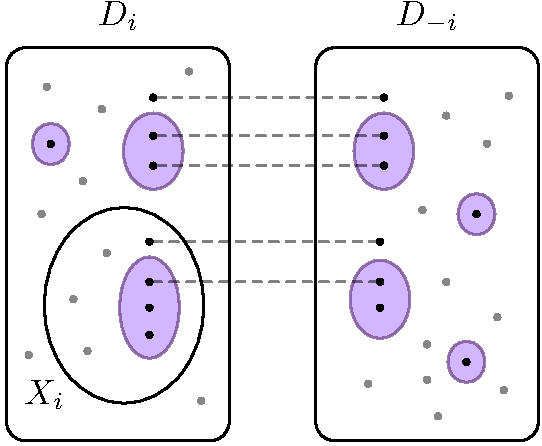
\includegraphics[scale=0.7]{figures/fig-efinf.pdf}
\caption{Elements of type $S$ have coloured background.}
\label{fig:efinf}
\end{figure}

First we prove that such a set $X_{-i}$ exists. 
To satisfy item~\eqref{it:piso} \eloise just needs to add to $X_{-i}$ the 
elements connected to $X_i$ by $f_n$; this is not a problem.

For item~\eqref{it:equiv} we proceed as follows: for every type $S$ such that 
there is an element $d\in X_i$ of type $S$, we add a new element $d'\in D_{-i}$
of type $S$ to $X_{-i}$. 
To see that this is always possible, observe first that $\osmodel_0 
\sim_k^\infty \osmodel_1$ implies $\osmodel_0 \sim_k^= \osmodel_1$. 
Using the properties of this relation, we divide in two cases:
%
\begin{itemize}
\item If $|S|_{D_i} \geq k$ we know that $|S|_{D_{-i}} \geq k$ as well. 
From the elements of $D_{-i}$ of type $S$, at most $n<k$ are used by $f_n$. 
Hence, there is at least one $d'\in D_{-i}$ of type $S$ to choose from.

\item If $|S|_{D_i} < k$ we know that $|S|_{D_{i}} = |S|_{D_{-i}}$. 
From the elements of $D_{i}$ of type $S$, at most $|S|_{D_{i}}-1$ are used by 
$f_n$. 
(The reason for the `$-1$' is that we are assuming that we have just chosen a 
$d\in X_i$ which is not in $f_n$.) 
Using that $|S|_{D_{i}} = |S|_{D_{-i}}$ and that $f_n$ is a partial isomorphism 
we can again conclude that there is at least one $d'\in D_{-i}$ of type $S$ to 
choose from.
\end{itemize}
	
Finally, we need to show that \eloise can choose $X_{-i}$ to be infinite.
To see this, observe that $X_{i}$ is infinite, while there are only finitely 
many types.
Hence there must be some $S$ such that $|S|_{X_i} \geq \omega$. 
It is then safe to add infinitely many elements for $S$ in $X_{-i}$ while 
considering point~\eqref{it:equiv}. 
Moreover, the existence of infinitely many elements satisfying $S$ in $D_{-i}$
is guaranteed by $\osmodel_0 \sim_k^\infty \osmodel_1$.

Having shown that \eloise can choose a set $X_{-i}$ satisfying the above 
conditions, it is now clear that using point~\eqref{it:equiv} \eloise can 
survive the ``first-order part'' of the second-order move we were considering.
This finishes the proof of the claim.
\end{pfclaim}

\noindent
Returning to the proof of Proposition~\ref{prop:connolque}, for 
step~(\ref{prop:connolque:iii}) to~(\ref{prop:connolque:i}) we prove the following.
	
\begin{claim}
Let $\vlist{s_i} \in D_i^n$ and $\phi(z_1,\dots,z_n) \in \ofoei(A)$ be such
that $\qr(\phi) \leq k-n$. 
If \eloise has a winning strategy in 
$\efgame_k^\infty(\osmodel_0,\osmodel_1)@(\vlist{s_0},\vlist{s_1})$ then 
$\osmodel_0 \models \phi(\vlist{s_0})$ iff 
$\osmodel_1 \models \phi(\vlist{s_1})$.
\end{claim}
	
\begin{pfclaim}
All the cases involving operators of $\ofoe$ are the same as in 
Proposition~\ref{prop:connofoe}. 
We prove the inductive case for the generalised quantifier. 
Let $\phi(z_1,\dots,z_n)$ be of the form $\qu x.\psi(z_1,\dots,z_n,x)$ and 
let $\osmodel_0 \models \phi(\vlist{s_0})$. 
Hence, the set $X_{0} \isdef \{ d_{0} \in D_{0} \mid \osmodel_0 \models 
\psi(\vlist{s_0},d_0) \}$ is infinite.

By assumption \eloise has a winning strategy in 
$\efgame_k^\infty(\osmodel_0,\osmodel_1)@(\vlist{s_0},\vlist{s_1})$.
Therefore, if \abelard plays a second-order move by picking $X_0 \subseteq D_0$
she can respond with some infinite set $X_1 \subseteq D_1$. 
We claim that 
$\osmodel_1 \models \psi(\vlist{s_1},d_1)$ for every $d_1\in X_1$. 
First observe that if this holds then the set $X'_1 \isdef  \{ d_1 \in D_1 \mid 
\osmodel_1 \models \psi(\vlist{s_1},d_1)\}$ must be infinite, and hence 
$\osmodel_1 \models \qu x.\psi(\vlist{s_1},x)$.


Assume, for a contradiction, that $\osmodel_1 \not\models \psi(\vlist{s_1},d'_1)$
for some $d'_1\in X_1$. 
Let \abelard play this $d'_1$ as the second part of his move. 
Then, as \eloise has a winning strategy, she will respond with some $d'_0 \in 
X_0$ for which she has a winning strategy in 
$\efgame_{k}^\infty(\osmodel_0,\osmodel_1)%
  @(\vlist{s_0}{\cdot}d'_0,\vlist{s_1}{\cdot}d'_1)$. 
But then by our induction hypothesis, which applies since $\qr(\psi) \leq
k-(n+1)$, we may infer from $\osmodel_1 \not\models \psi(\vlist{s_1},d'_1)$
that $\osmodel_0 \not\models \psi(\vlist{s_0},d'_0)$.
This clearly contradicts the fact that $d'_{0} \in X_{0}$.
\end{pfclaim}
	
\noindent
Combining the claims finishes the proof of the proposition.
\end{proof}


\begin{theorem}
\label{thm:bfofoei}
There is an effective procedure that transforms an arbitrary $\ofoei$-sentence 
$\phi$ into an equivalent formula $\tbas{\phi}$ in basic form.
\end{theorem}

\begin{proof}
This can be proved using the same argument as in Theorem~\ref{thm:bnfofoe} but
based on Proposition \ref{prop:connolque}. 
Hence we only focus on showing that $\phi_E^\infty \equiv 
\dbnfofoei{\vlist{T}}{\Pi}{\Sigma}$ for some 
$\vlist{T},\Pi,\Sigma \subseteq \wp(A)$ such that $\Sigma \cup \Pi \subseteq
\vlist{T}$, where $\phi_E^\infty$ is the sentence characterising
$E \in \umods/{\sim^\infty_k}$ from 
Proposition \ref{props:eqrelolque}(\ref{props:eqrelofoe:ii}). 
Recall that
\[
\phi^\infty_E = \phi^=_{E'} \land \dbnfinf{\Sigma}
\]
where $\Sigma$ is the collection of types that are realised by infinitely many 
elements.
Using Theorem~\ref{thm:bnfofoe} on $\phi^=_{E'}$ we know that this is 
equivalent to
\[
\phi^\infty_E = \dbnfofoe{\vlist{T}}{\Pi'} \land \dbnfinf{\Sigma}
\]
where $\Pi' \subseteq \vlist{T}$.
Observe that we may assume that $\Sigma \subseteq \Pi$, otherwise the formula 
would be inconsistent.
Now separate $\Pi'$ as $\Pi' = \Pi \uplus \Sigma$ where $\Pi \isdef 
\Pi'\setminus\Sigma$ consists of the types that are satisfied by finitely many 
elements.
Then we find 
\[
\phi^\infty_E \equiv 
\dbnfofoe{\vlist{T}}{\Pi\cup\Sigma} \land \dbnfinf{\Sigma}.
\]
Therefore, we can conclude that $\phi^\infty_E \equiv 
\dbnfofoei{\vlist{T}}{\Pi}{\Sigma}$.
\end{proof}

\noindent
The following slightly stronger normal form will be useful in later 
chapters.

\begin{proposition}\label{prop:bfofoei-sigmapi}
For every sentence in the basic form $\bigvee \dbnfofoei{\vlist{T}}{\Pi}{\Sigma}$
it is possible to assume, without loss of generality, that $\Sigma \subseteq 
\Pi \subseteq \vlist{T}$.
\end{proposition}
\begin{proof}
This is direct from observing that $\dbnfofoei{\vlist{T}}{\Pi}{\Sigma}$ is 
equivalent to $\dbnfofoei{\vlist{T}}{\Pi\cup\Sigma}{\Sigma}$. 
To check it we just unravel the definitions and observe that
$\dbnfofoe{\vlist{T}}{\Pi \cup \Sigma} \land \dbnfinf{\Sigma}$ is equivalent to
$\dbnfofoe{\vlist{T}}{\Pi \cup \Sigma \cup \Sigma} \land \dbnfinf{\Sigma}$.
\end{proof}
